%%%%%%%%%%%%%%%%%%%%%%%%%%%%%%%%%%%%%%%%%%%%%%%%%%%%%%%%%%%%%%%%%%%%%%%%%%%
%% This file is part of the book
%%
%% Algorithmic Graph Theory
%% http://code.google.com/p/graph-theory-algorithms-book/
%%
%% Copyright (C) 2009--2011 Minh Van Nguyen <nguyenminh2@gmail.com>
%%
%% See the file COPYING for copying conditions.
%%%%%%%%%%%%%%%%%%%%%%%%%%%%%%%%%%%%%%%%%%%%%%%%%%%%%%%%%%%%%%%%%%%%%%%%%%%

\documentclass{article}

\usepackage{tikz}
\usetikzlibrary{external}
\usetikzlibrary{trees}
\tikzexternalize{tree-traversal}

\begin{document}

\begin{figure}
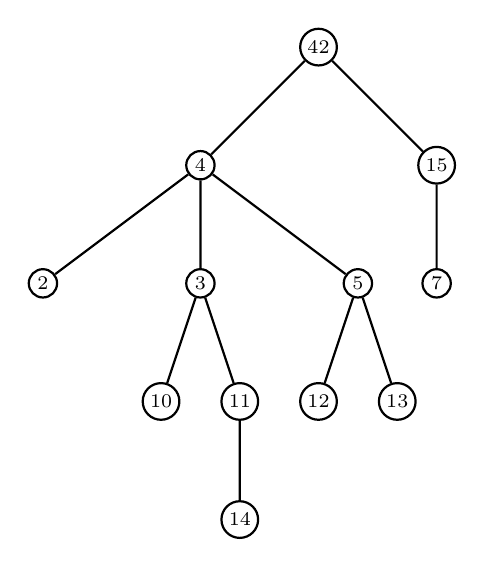
\begin{tikzpicture}
[-,thick,%
  every node/.style={shape=circle,inner sep=1.5pt,draw,thick}]
\scriptsize
\node {$42$}
  [sibling distance=3cm]
  child {node {$4$}
    [sibling distance=2cm]
    child {node {$2$}}
    child {node {$3$}
      [sibling distance=1cm]
      child {node {$10$}}
      child {node {$11$}
        child {node {$14$}}
      }
    }
    child {node {$5$}
      [sibling distance=1cm]
      child {node {$12$}}
      child {node {$13$}}
    }
  }
  child {node {$15$}
    [sibling distance=2cm]
    child {node {$7$}}
  };
\end{tikzpicture}
\end{figure}

\end{document}
